% --------------------------------------------------------------
% This is all preamble stuff that you don't have to worry about.
% Head down to where it says "Start here"
% --------------------------------------------------------------

\documentclass[12pt]{article}

\usepackage[margin=1in]{geometry} 
\usepackage{amsmath,amsthm,amssymb}
\usepackage{color}
\usepackage{tikz, pgfplots}
\usepackage{graphicx}
\usepackage{epstopdf} %converting to PDF
\usepackage{subcaption}

\makeatletter

\renewcommand\section{\@startsection {section}{1}{\z@}%
	{-3.5ex \@plus -1ex \@minus -.2ex}%
	{2.3ex \@plus.2ex}%
	{\normalfont\large\bfseries}}% from \Large
\renewcommand\subsection{\@startsection{subsection}{2}{\z@}%
	{-3.25ex\@plus -1ex \@minus -.2ex}%
	{1.5ex \@plus .2ex}%
	{\normalfont\large\bfseries}}% from \large
\makeatother

\begin{document}
	
	% --------------------------------------------------------------
	%                         Start here
	% --------------------------------------------------------------
	
	%\renewcommand{\qedsymbol}{\filledbox}
	
	\title{\textbf{Machine Learning Assignment \#2}\\
	Universit{\"a}t Bern}%replace X with the appropriate number
	\author{Lin Bai 09935404} %replace with your name
	
	\maketitle
	
	%%%%%%%%%%%%%%%%%%%%%%%%%%%%%%%%%%%%%%%%%%%%%%%%%%%%%%%%%%%%%%%%%%%%%%%%%%%%%%%%%%%%%%%%
	%%%%%%   notations
	%%%%%%%%%%%%%%%%%%%%%%%%%%%%%%%%%%%%%%%%%%%%%%%%%%%%%%%%%%%%%%%%%%%%%%%%%%%%%%%%%%%%%%%%
%	\section*{notations}
%	$A, B, C\in \mathbb{R}^{n\times n}$ are $n\times n$ matrices, $x, a, b\in \mathbb{R}^n$ are column vectors.

	%%%%%%%%%%%%%%%%%%%%%%%%%%%%%%%%%%%%%%%%%%%%%%%%%%%%%%%%%%%%%%%%%%%%%%%%%%%%%%%%%%%%%%%%
	%%%%%%   question 1
	%%%%%%%%%%%%%%%%%%%%%%%%%%%%%%%%%%%%%%%%%%%%%%%%%%%%%%%%%%%%%%%%%%%%%%%%%%%%%%%%%%%%%%%%
	\section*{Solution of question 1}
	1. \textbf{Train the SVM classifier with different choices of the regularization parameter $\lambda$. Plot a graph where you show the classification performance versus $\lambda$. What is the optimal regularization parameter?}\\
	\noindent
	In order to find the optimal value of $\lambda$, first, the sweep of lambda in a large range is done. Start from $10^{-4}$ to $10^6$, then we get figure 1 shown below. This curve is plotted in log scale.\\
	
	%%%%%%%%%%%%%%%%%%%%%%%%%%%%%%%
	%%% FIGURE 1
	%%%%%%%%%%%%%%%%%%%%%%%%%%%%%%%	
	\begin{figure}[!htb]
		\centering
		\includegraphics[scale=.7]{lambda_n8to0}
		\caption{lambda sweep from $10^{-8}$ to $10^{-1}$}
		\label{fig:lambdaLargeSweep}
	\end{figure}
	\noindent
	Where we could find the optimal value of $\lambda$ is round 0.0001.\\
	Then further check is done for range from $10^{-4}$ to $10^{-3}$ in Figure \ref{fig:lambda4to3} and range from $10^{-3}$ to $10^{-2}$ in Figure \ref{fig:lambda3to2}. From the figure, we know when $\lambda=0.0004$ the accuracy is highest.\\
	
	%%%%%%%%%%%%%%%%%%%%%%%%%%%%%%%
	%%% FIGURE 2
	%%%%%%%%%%%%%%%%%%%%%%%%%%%%%%%	
	\begin{figure}
		\begin{subfigure}{.5\textwidth}
			\centering
			\includegraphics[width=.9\linewidth]{lambda_n4ton3}
			\caption{from $10^{-4}$ to $10^{-3}$}
			\label{fig:lambda4to3}
		\end{subfigure}%
		\begin{subfigure}{.5\textwidth}
			\centering
			\includegraphics[width=.9\linewidth]{lambda_n3ton2}
			\caption{from $10^{-3}$ to $10^{-3}$}
			\label{fig:lambda3to2}
		\end{subfigure}
		\caption{lambda sweep in detail}
		\label{fig:fig}
	\end{figure}
	\noindent
	P.S:- Due to the fact that each time we run the exercise1.m, the accuracy varies. Therefore the average of 10 times running is used in the analysis and plotting.\\
	\\
	2. \textbf{Compare SVM to the previously implemented learning algorithms (logistic regression and GDA) in terms of classification accuracy.}\\
	From the classification accuracy point of view, SVM's performance(0.8324) is better than SGD(0.7039) and GDA(0.7353).\\
	
	%%%%%%%%%%%%%%%%%%%%%%%%%%%%%%%%%%%%%%%%%%%%%%%%%%%%%%%%%%%%%%%%%%%%%%%%%%%%%%%%%%%%%%%%
	%%%%%%   question 2
	%%%%%%%%%%%%%%%%%%%%%%%%%%%%%%%%%%%%%%%%%%%%%%%%%%%%%%%%%%%%%%%%%%%%%%%%%%%%%%%%%%%%%%%%
	\section*{Solution of question 2}
	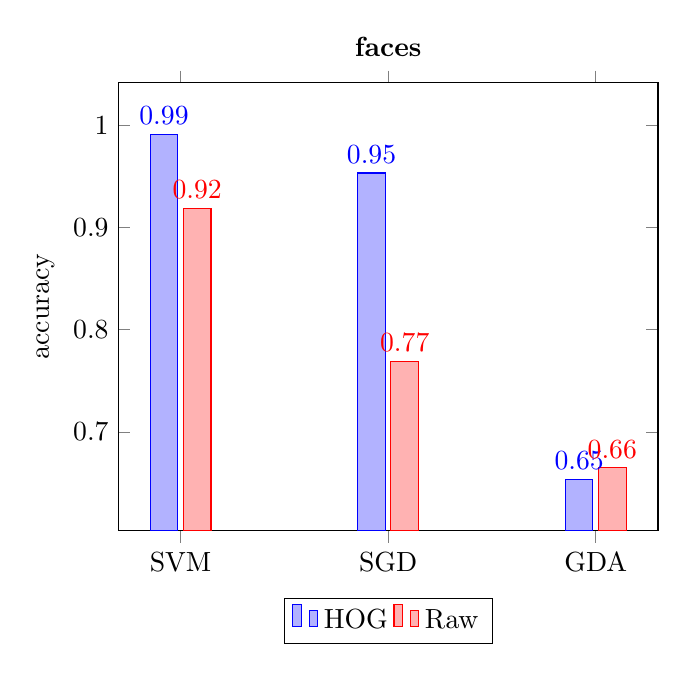
\begin{tikzpicture}
	\centering
	\begin{axis}[
	title={\textbf{faces}},
	ybar,
	enlargelimits=0.15,
	legend style={at={(0.5,-0.15)},
		anchor=north,legend columns=-1},
	ylabel={accuracy},
	symbolic x coords={SVM,SGD,GDA},
	xtick=data,
	nodes near coords,
	nodes near coords align={vertical},
	]
	\addplot coordinates {(SVM,0.99109) (SGD,0.9532) (GDA,0.6539)};
	\addplot coordinates {(SVM,0.91840) (SGD,0.7693) (GDA,0.6648)};
	\legend{HOG, Raw}
	\end{axis}
	\end{tikzpicture}
	\noindent
	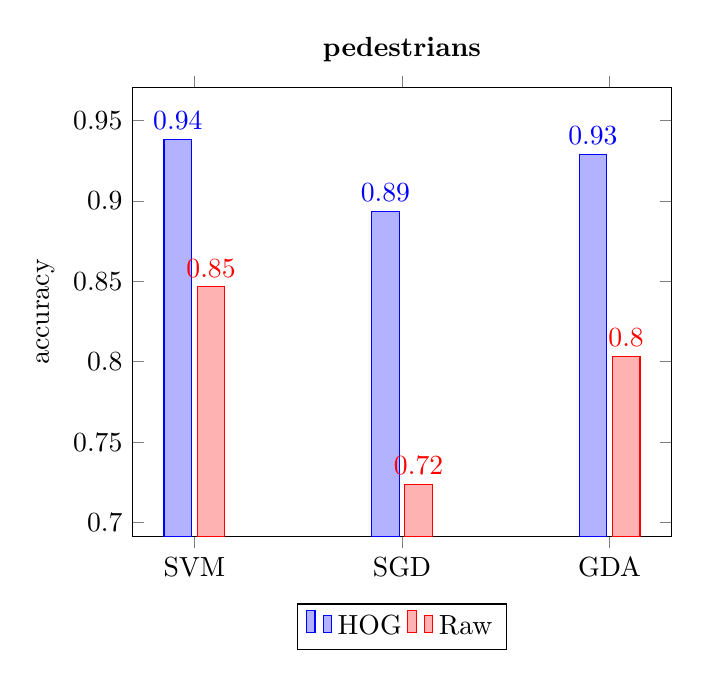
\begin{tikzpicture}
	\centering
	\begin{axis}[
	title={\textbf{pedestrians}},
	ybar,
	enlargelimits=0.15,
	legend style={at={(0.5,-0.15)},
		anchor=north,legend columns=-1},
	ylabel={accuracy},
	symbolic x coords={SVM,SGD,GDA},
	xtick=data,
	nodes near coords,
	nodes near coords align={vertical},
	]
	\addplot coordinates {(SVM,0.93807) (SGD,0.8933) (GDA,0.9290)};
	\addplot coordinates {(SVM,0.84656) (SGD,0.7237) (GDA,0.8033)};
	\legend{HOG, Raw}
	\end{axis}
	\end{tikzpicture}
	\\
	\noindent
	1. \textbf{Compare the HOG features to the raw pixels. Which feature representation	is better for classification?}\\
	In order to find out the better feature representation for classification, we introduce accuracy-speed product(ASP) to evaluate.\\
	$$ASP = \frac{accuracy[percentage]}{time\_cost[second]}$$
	Take SVM and faces for example, when HOG is used, the accuracy(average of 10) is  0.9895, and the time cost is 20.51121 seconds. It's ASP is 0.048. On the other hand, when raw pixel is used, the accuracy(average of 10) is 0.9180, and the time cost is 9.893387 seconds. It's ASP is 0.093.\\
	Therefore, raw pixel is better for classification from accuracy-speed product point of view.\\
	\\
	\noindent
	2. \textbf{Compare the training algorithms (SVM, logistic regression and GDA) in terms of classification accuracy.}\\
	From the plot, no matter which feature representation is chosen, SVM always achieves the best performance.\\
	\\
	\noindent
	3. \textbf{According to the experiments what is more important? The learning algorithm, or the feature representation?}\\
	\\
	\noindent
	4. \textbf{On which dataset do HOG features help more? Justify your answer.}\\
	From the figures above, HOG has better performance when used for faces.\\
	Because the pedestrians are varies from each other due to their gestures. And this difference is larger in pedestrians dataset when comparing to faces dataset.\\

	%%%%%%%%%%%%%%%%%%%%%%%%%%%%%%%%%%%%%%%%%%%%%%%%%%%%%%%%%%%%%%%%%%%%%%%%%%%%%%%%%%%%%%%%
	%%%%%%   question 3, sub question (a)
	%%%%%%%%%%%%%%%%%%%%%%%%%%%%%%%%%%%%%%%%%%%%%%%%%%%%%%%%%%%%%%%%%%%%%%%%%%%%%%%%%%%%%%%%
	\section*{Solution of question 3}
	1. \textbf{Before you run the experiment, what kind of performance do you expect from the raw pixels and the HOG features (in terms of average precision)?}\\
	The expected performance is, \\
	when HOG features is used, this experiment will achieve higher accuracy than exercise1. However, when raw pixel is chosen, the accuracy of two exercise are similar.\\
	\\
	\noindent
	2. \textbf{What is the difference between the performances on the dataset used previously and the dataset used in this experiment? Explain why you get these results.}\\
	 

	%%%%%%%%%%%%%%%%%%%%%%%%%%%%%%%%%%%%%%%%%%%%%%%%%%%%%%%%%%%%%%%%%%%%%%%%%%%%%%%%%%%%%%%%
	%%%%%%   question 3, sub question (a)
	%%%%%%%%%%%%%%%%%%%%%%%%%%%%%%%%%%%%%%%%%%%%%%%%%%%%%%%%%%%%%%%%%%%%%%%%%%%%%%%%%%%%%%%%
	\section*{Solution of question 4}
	%%%%%%%%%%%%%%%%%%%%%%%%
	
	% --------------------------------------------------------------
	%     You don't have to mess with anything below this line.
	% --------------------------------------------------------------
	
\end{document}
